\documentclass{uai2025} % for initial submission
%\documentclass[accepted]{uai2025} % after acceptance, for a revised version; 
% also before submission to see how the non-anonymous paper would look like 
                        
%% There is a class option to choose the math font
% \documentclass[mathfont=ptmx]{uai2025} % ptmx math instead of Computer
                                         % Modern (has noticeable issues)
% \documentclass[mathfont=newtx]{uai2025} % newtx fonts (improves upon
                                          % ptmx; less tested, no support)
% NOTE: Only keep *one* line above as appropriate, as it will be replaced
%       automatically for papers to be published. Do not make any other
%       change above this note for an accepted version.

%% Choose your variant of English; be consistent
\usepackage[american]{babel}
% \usepackage[british]{babel}

%% Some suggested packages, as needed:
\usepackage{natbib} % has a nice set of citation styles and commands
    \bibliographystyle{plainnat}
    \renewcommand{\bibsection}{\subsubsection*{References}}
\usepackage{mathtools} % amsmath with fixes and additions
% \usepackage{siunitx} % for proper typesetting of numbers and units
\usepackage{booktabs} % commands to create good-looking tables
\usepackage{tikz} % nice language for creating drawings and diagrams

\usepackage{amsmath}
\usepackage{amssymb}
\usepackage{amsthm}
\usepackage{todonotes}
\usepackage{bm}
\usepackage{subcaption}
\usepackage{fancyvrb}
\usepackage[ruled]{algorithm2e}

\def\ci{\perp\!\!\!\!\!\perp}

\newtheorem{definition}{Definition}
\newtheorem{proposition}{Proposition}
\newtheorem{theorem}{Theorem}

\title{Expert-In-The-Loop Causal Discovery: Iterative Model Refinement Using Expert Knowledge}

% The standard author block has changed for UAI 2025 to provide
% more space for long author lists and allow for complex affiliations
%
% All author information is authomatically removed by the class for the
% anonymous submission version of your paper, so you can already add your
% information below.
%
% Add authors
\author[1]{\href{mailto:<ankur.ankan@ru.nl>?Subject=Your UAI 2025 paper}{Ankur~Ankan}{}}
\author[1]{Johannes~Textor}

% Add affiliations after the authors
\affil[1]{%
    Institute for Computing and Information Sciences\\
    Radboud University\\
    Nijmegen, The Netherlands
}
\begin{document}

\maketitle

\begin{abstract}
% Causal discovery has received significant attention in the Directed Acyclic
% Graphs (DAGs) literature, leading to the development of numerous automated
% algorithms for learning DAGs from data. Despite these advancements, the
% application of these algorithms in applied domains remains limited, with
% researchers often preferring to manually construct DAGs based on their expert
% knowledge. This preference stems due to some practical issues with these
% algorithms such as making obvious mistakes, and outputting Markov Equivalence
% Class (MEC). As a result of these issues users typically have to rely on post
% hoc modifications to the model based on their expertise. Given this reliance on
% manual model modification and construction, we propose an iterative method to
% assist researchers in manually constructing DAGs by combining implied
% Conditional Independence (CI) based model testing and utilizing their expert
% knowledge. We present a novel measure of partial association for mixed data
% that allows us to rank violations of implied CIs in the model. Using this
% ranking users can prioritize modifications to the model while using their
% expert knowledge to decide orientation of edges. Empirically, we show that
% a greedy approach achieves performance comparable to automated algorithms, provided
% the user can correctly determine the edge orientation in $ 1 $ out of $ 3 $ cases.
% Additionally, we show that in the absence of an expert, a Large Language Model can
% potentially be used for determining edge orientations.

Causal discovery has received significant attention in the Directed Acyclic
Graphs (DAGs) literature, leading to the development of numerous automated
algorithms for learning DAGs from data. However, their adoption in applied
domains remain limited, as researchers often prefer to construct DAGs manually
based on their domain knowledge. This preference arises due to several
practical issues with automated algorithms, such as they make obvious errors
and output Markov Equivalence Classes (MECs). To address these challenges, we
propose an iterative method to assist researchers in manually constructing or
improving an existing DAG by combining implied Conditional Independence (CI)
testing with expert knowledge. Our proposed method utilizes a novel measure of
partial association for mixed data to rank violations of implied CIs in a given
DAG, enabling users to prioritize modifications while utilizing their domain
knowledge to decide the orientation of new edges. Empirical results show that
this manual model construction approach achieves performance comparable to
automated algorithms if the user is able correctly orientation edges in one out
of three cases. Additionally, we demonstrate that, in the absence of an expert,
a Large Language Model (LLM) can be potentially determine edge orientations. We
provide the implementation of our approach in both a web tool at: <redacted for
review> and a Python package <redacted for review>.

\end{abstract}

\section{Introduction}
Understanding cause-and-effect relationships between variables is a fundamental
objective in many scientific fields. These relationships reveal the mechanisms
behind observed phenomena and guide effective interventions or policy
decisions. \emph{Causal Discovery} methods aim to discover such relationships
among random variables using observational data. Approaches to causal discovery
have been developed within both the Directed Acyclic Graphs (DAGs) and
Structural Equation Models (SEMs) frameworks, each adapting a different
approach.

In the DAG literature, the primary focus has been on developing automated
algorithms to learn causal structures from datasets. These efforts have led to
numerous causal discovery algorithms, including constraint-based methods like
the PC algorithm \citep{Spirtes2001} and Fast Causal Inference (FCI)
\citep{Spirtes2000}), score-based methods such as Hill-Climb Search and Greedy
Equivalence Search (GES) \citep{Chickering2002}, and continuous
optimization-based methods like NO TEARS \citep{Zheng2018} and DAGMA
\citep{Bello2022}. While DAG-based methods focus on automated discovery,
SEM-based methods emphasize expert-driven model specification. This includes
tools to assist researchers in manually constructing models, enabling them to
incorporate their domain knowledge in the model building process. Researchers
typically begin with an initial model based on their expertise and then use
these tools to guide modifications that improve the model's fit to data. This
process is commonly known as \emph{Specification Search} \citep{Long1983} and
uses method such as modification indices, and Wald-based tests
\citep{Marcoulides2018}. 

Despite significant progress in automated causal discovery, their adoption in
applied research has been limited. Researchers often prefer to manually
construct DAGs based on their domain expertise \citep{Tennant2020,
Petersen2021}. We attribute this preference to several challenges with existing
causal discovery algorithms in practical settings:

\begin{enumerate}
	\item \textbf{Lack of Trust:} While most algorithms are asymptotically
		consistent, their behavior on finite samples is not well
		understood. Additionally, their output can vary significantly
		depending on the choice of algorithm and hyperparameters,
		making it difficult to assess reliability. The absence of
		robust performance evaluation methods for any given dataset
		further reduce the confidence in their outputs. 
	\item \textbf{Outputs Markov Equivalence Class (MEC):} As multiple
		DAGs can be faithful to a given observational dataset, automated 
		algorithms can only recover the MECs. These MECs can contain a
		combination of directed and undirected edges. However, most
		methods for downstream tasks, such as identification or causal
		effect estimation, assume knowledge of a fully oriented DAG. 
\end{enumerate}

Fig.~\ref{fig:intro} highlights some of these issues. When constructing models
manually it is important to test whether the constructed DAG is representative
of the dataset or not. Based on this testing and domain knowledge further
modifications can be made to the DAG. One of the approaches to test and modify
DAGs is by testing whether the implied CI tests of the DAG are true in the data
or not \citep{Ankan2021}. If some of the tests are violated in the data,
researchers can use their domain knowledge to make modifications to the DAG.

However, this CI testing approach also has a few drawbacks: 1) CIs are implied
only by missing edges in the model, so we can not test whether the existing
edges are correct or not. 2) The decision whether a CI holds in the data or not
is based on a p-value threshold. But we can get significant p-values for even
very weak relationship if the sample size is high. 3) Lastly, the number of
implied CIs can be large making it difficult to go through all of them; for 
example, in the moderately sized alarm network \citep{Beinlich1989} with $ 37 $
nodes, there are $ 287 $ implied CIs.


% To deal with these issues
% methods for integrating expert knowledge have been developed. The two main
% methods to integrate expert knowledge in the model construction process is to:
% 1. Provide all the expert knowledge to the causal discovery algorithm for
% example in the form of required and forbidden edges \citep{Meek1995}, or
% temporal information \citep{Bang2023} and let the algorithm use it to construct
% the model. 2. Utilize conditional independence (CI) testing to identify issues in
% the model, and manually fix them based on expert knowledge \citep{Ankan2021}.
% We focus on this second approach in this paper.

% In this CI testing procedure, users test whether the implied CIs of the DAG
% hold in the dataset or not using statistical CI tests. Based on the results of
% these statistical tests, we can accordingly make modifications to the current
% model to fix the violations. However, this CI based testing also has a few
% drawbacks: 1) CIs are implied only by missing edges in the model, so we can not
% test for already existing edges. 2) In high sample size scenarios, p-values can
% suggest a significant association between variables even if they have a very
% weak relationship. 3) Number of implied CIs can be large making it difficult to
% manually go through each of them; for example, in the moderately sized alarm
% network with $ 37 $ node, there are $287$ implied CIs. 

% There has been work on trying to come up with a single test to combine all
% these test to give a single answer \citep{Eulig2023, Shipley2000}. However,
% what is missing is the guide on how to how to fix these tests. Additionally
% there has been a lot of work to integrate expert knowledge into causal
% discovery algorithms which has shown significant improvement. 

To tackle these issues with CI based testing, we take inspiration from
\emph{modification indices} in specification search. The modification indices
method tries to identify and rank changes in the model such that modifications
that improve the model fit the most are ranked higher. This ranking allows
researchers to focus first on the suggestions that can improve the model the
most and while integrating their expertise to choose the most optimal
modifications. Analogous to this, we develop a procedure for ranking CI test
violations allowing researchers to focus on the worst violations in the model.
This ranking method utilizes both p-values and a measure of conditional
association. Utilizing this procedure researchers can iteratively construct
DAGs while integrating their domain knowledge in the model building procedure.

\begin{figure}[t!]
\begin{subfigure}{0.25 \textwidth}
	\includegraphics[page=1]{figures.pdf}
	\caption{$ N = 400 $}
\end{subfigure}%
\begin{subfigure}{0.25 \textwidth}
	\includegraphics[page=2]{figures.pdf}
	\caption{$ N = 800$ }
\end{subfigure}
\begin{subfigure}{0.25 \textwidth}
	\includegraphics[page=5]{figures.pdf}
	\caption{$ N = 400 $ }
\end{subfigure}%
\begin{subfigure}{0.25\textwidth}
	\includegraphics[page=6]{figures.pdf}
	\caption{ $ N = 800$ }
\end{subfigure}
\begin{subfigure}{0.25 \textwidth}
	\includegraphics[page=3]{figures.pdf}
	\caption{ $ N = 400$ }
\end{subfigure}%
\begin{subfigure}{0.25\textwidth}
	\includegraphics[page=4]{figures.pdf}
	\caption{$ N = 800$ }
\end{subfigure}

\caption{A comparison of Markov Equivalence Class (MEC) learned using Adult Income Dataset \citep{Becker1996} using (a \& b) PC algorithm using a mutual information based test, (c \& d) Hill Climb Search with Bayesian Information Criterion (BIC) score, (e \& f) PC algorithm with a residualization based test \citep{Ankan2023}. The learned model structure varies significantly depending on the algorithm, the CI test, and the sample size used.}
\label{fig:intro}
\end{figure}


Our main contributions in this paper are as follows:
\begin{enumerate}
	\item We propose a novel measure of conditional association for mixed data
		based on canonical correlations. This measure of association
		generalizes some of the commonly used special case measures of 
		association to mixed data.
	\item Using this conditional association measure, we present a procedure to
		manually construct DAGs by ranking violation of implied CIs in the 
		model. This iterative procedure allows users to integrate their
		domain knowledge in the model construction procedure.
	\item Lastly, to allow researchers to easily apply this method on their
		datasets, we present a web-browser based interactive tool as well
		as implementation in a Python package.
\end{enumerate}

The rest of the paper is structured as follows. In
Section~\ref{sec:background}, we give a background on the commonly used
measures of association for various data types. In
Section~\ref{sec:mixed_association}, we present our generalized measure of
conditional association for mixed data. Section~\ref{sec:modification} provides
details on the procedure for using the measure of association for constructing
DAGs. Section~\ref{sec:web} presents our web-browser based tool and lastly in
Section~\ref{sec:empirical}, we show some empirical results to compare this
manual DAG construction approach to automated algorithms.

\section{Background and Related Work}
\label{sec:background}
\subsection{Notations}
\todo[inline]{Improve this section once all the notations are in place}
We denote random variables with uppercase letters $ X $, and a set of random
variables as $ \bm{X} = \{X_1, \cdots, X_k\} $ with $ \rvert \bm{X} \rvert = k
$. A sample from the random variable $ X $ is denoted as $ x $ and from a set
of random variables $ \bm{X} $ is denoted as $ \bm{x} $. In this paper, we
consider random variables in the mixed data setting where each of the random
variables can be either of continuous, categorical, or ordinal unless
specified. We write the expectation of a variable $ X $ as $ \mathbb{E}[X] $, conditional
expectations as $ \mathbb{E}[X | \bm{Z}] $.

\subsection{Measures of Conditional Association}
Our proposed method for iterative DAG construction relies on a measure of
conditional association also known as partial association between variables. We
are interested in measuring the association between variables $ X $ and $ Y $
when conditioned on a set of variables $ \bm{Z} $ which is potentially an empty
set, $ \bm{Z} = \emptyset $. Many special case measures of conditional
association have been used in literature depending on the type of $ X $, $ Y $,
and $ \bm{Z} $. Typically, these are the effect size measures of the CI test $
X \ci Y \rvert \bm{Z} $. In this section, we give an overview of some of the
commonly used measures for different data types.

\todo[inline]{Remove or move equations to appendix if no space}

\subsubsection{Both $ X $ and $ Y $ are continuous}
When both $ X $ and $ Y $ are continuous variables, Pearson's correlation
coefficient is typically used. In the case when $ \bm{Z} = \emptyset $, the
correlation coefficient is given as:

\begin{equation}
\rho_{X, Y} = \frac{\mathrm{cov}(X, Y)}{\sigma_X \sigma_Y}
\end{equation}

where $ \mathrm{cov}(X, Y) $ is the covariance between $ X $ and $ Y $, and $
\sigma_X $ and $ \sigma_Y $ are the standard deviations of $ X $ and $ Y $
respectively. When $ \bm{Z} \neq \emptyset $, partial correlation coefficient
can be used. One of the ways to estimate it is to use two linear regression
models: 

\begin{equation}
	\begin{split}
		E_X &: X \sim \bm{Z} \\
		E_Y &: Y \sim \bm{Z} \\
		\rho_{X, Y; \bm{Z}} &= \frac{cov((X - E_X), (Y - E_Y))}{\sigma_{(X - E_X)} \sigma_{(Y-E_Y)}}
	\end{split}
\end{equation}

$ E_X: x \sim \bm{z} $, and $ E_Y: y \sim \bm{z} $. Then we take the compute
the Pearson's correlation coefficient between the residuals of these two
regressions: $ R_X = x - E_X(\bm{z}) $, $ R_Y = y - E_Y(\bm{z}) $.

\paragraph{All $ X $, $ Y $, and $ \bm{Z} $ are discrete}

In the case of discrete variables, Cramer\'s V has been typically used as a
measure of association. When there are no conditional variables, $ \bm{Z} =
\emptyset $, Cramer\'s V can be computed directly from the contingency table.

However, when conditional variables are present, we can iterate over all
possible combinations of the conditional variables, compute the Cramer\'s V and
then lastly combine them together. 

\paragraph{$ X $ is ordinal and $ Y $ is continuous or ordinal}
Polyserial Correlation (when one is oridinal and the other is continuous) and
polychoric correlation (when both are ordinal) can be use. Here the assumption
is made that $ X $ is a thresholded version of an underlying continuous normal
variable. The method then tries to learn the thresholds for this latent
variable while trying to maximize the correlation between $ X_{lat} $ and $ Y
$. This gives us values that are Pearson's correlation coefficient.

\section{A Generalized Measure of Conditional Association}
\label{sec:mixed_association}

In the previous section, we discussed how different types of variables require
different conditional measures of association. However, no unified measure
exists for mixed data. In this section, we introduce a novel measure of partial
association for mixed data, by extending the idea of partial correlation
coefficient to mixed data. Specifically, our approach combines a mixed data
residualization method \citep{Ankan2023} with Pillai's Trace
\citep{Pillai1955}, a multivariate measure of association based on canonical
correlations.
 
% As there are no generalized measures of association for mixed data, in this
% section, we first introduce a novel measure of partial association for mixed
% data by extending the concept of partial correlations \citep{Whittaker2009}
% \todo{Verify this citation} to handle mixed data types. To compute partial
% correlations, we have two key steps: 1) a residualization method, and 2) a
% measure of associations between the residuals. When both $ X $ and $ Y $ are
% continuous variables, residuals are typically computed using a regression-based
% method, and Pearson's correlation coefficient is used to measure the
% association between these residuals. To extend this approach to mixed data, we
% combine a mixed data residualization method \citep{Ankan2023} with a
% multivariate measure of association based on canonical correlations, Pillai's
% Trace \citep{Pillai1955}. 

Given $ n $ samples $ D = (x, y, \bm{z}) $ of variables $ X $, $ Y $, and $
\bm{Z} $, we aim to estimate the conditional association $ \rho(X, Y; \bm{Z}) $
between $ X $ and $ Y $ conditioned on $ \bm{Z} $. We first use the
residualization approach from \citet{Ankan2023} to compute the residual
matrices for both $ X $ and $ Y $. For each of the variable $ X $ and $ Y $, we
compute the residual $ R_X $ and $R_Y$ respectively as follows depending on
their type.

\begin{enumerate}
	\item \textbf{Continuous:} We train a regression model, $ E_X: x \sim
		\bm{z} $. The residuals are then defined as the difference
		between the true and the predicted values using $ E_X $. 
		$$ R_{x_i} = x_i - E_X(\bm{z}_i) $$
	\item \textbf{Ordinal:} We start by training a probability estimator, $
		p_X: x \sim \bm{z} $, and obtain probability predictions 
		$ \hat{p}_X: \hat{p}_X(\bm{Z}) $. Then, we compute the residuals
		as follows \citep{Li2012}:
		$$ R_{x_i} = \hat{p}(\hat{x}_i > x_i) - \hat{p}(\hat{x}_i < x_i) $$
	\item \textbf{Categorical:} We again start by training a probability
		estimator $ p_X: X \sim \bm{Z} $, and obtain probability
		estimates $ \hat{p}_X: p_Z(\bm{Z}) $. Next, we dummy encode the
		categorical variable and then compute the residuals as follows: 
		$$ R_X = x_i - \hat{p}(\bm{z}_i) $$
\end{enumerate}

\todo[inline]{Fix notations above}

We repeat the above steps for both the variables $ X $ and  $ Y $ to get
residuals $ R_X $ and $ R_Y $. Here, we have the option to choose the
estimators based on the properties of the data. Non-parametric ensemble
estimators such as Random Forest and XGBoost can handle any combination of data
types while performing reasonably well. For linear datasets, we can also choose
variants of linear regression depending on the type of data. 

After the above steps are repeated for both $ X $ and $ Y $, we end up with two
residual matrices: $ R_X $ and $ R_Y $. The type of the variable determines the
shape for these matrices. If the variable is continuous, we get a residual
matrix of shape $ ( n \times 1 ) $ and if the variable is categorical, we have
a residual matrix of shape $ ( x \times (k -1)) $ where one of the dummy encoded
variables is dropped to avoid multicollinearity.

We now have two continuous-valued residual matrices. The next step is
to quantify the association between these residuals. In multivariate
statistics, canonical correlation based measures have been used to measure
the association between two sets of variables. We can treat our residuals
as sets of variables and use canonical correlations to quantify the association
between them.

\begin{definition} 

	Given two sets of random variables $ \bm{U} = (U_1, U_2, \cdots, U_p) $
	and $ \bm{V} = (V_1, V_2, \cdots, V_q) $, canonical correlation between
	them, $\rho(\bm{U}, \bm{V}) $ is defined as:
		
	% \begin{equation}
	% 	\phi(\bm{U}, \bm{V}) = \sup_{a, b} \frac{a^T \Sigma_{\bm{U}\bm{V}} b}{\sqrt{a^T \Sigma_{\bm{U}\bm{U}} a} \sqrt{b^T \Sigma_{\bm{V}\bm{V}} b}}
	% \end{equation}

% \begin{equation}
% 	\begin{split}
% 		\bm{\rho}(\bm{U}, \bm{V}) &= \sqrt{\mathrm{E} \left( \Sigma_{\bm{UU}}^{-1} \Sigma_{\bm{UV}} \Sigma_{\bm{VV}}^{-1} \Sigma_{\bm{VU}} \right)}
% 	\end{split}
% \end{equation}
	\begin{equation}
		\rho(\bm{U}, \bm{V}) = \max_{a, b} Corr(a^T \bm{U}, b^T \bm{V})
	\end{equation}

	where $ a $ and $ b $ are vectors of coefficients that maximize the correlations
	between the linear combinations of $ a^T \bm{U} $ and $ b^T \bm{V} $.
\end{definition}

% where $ \mathrm{E}(\Sigma) $ denotes the eigenvalues of the matrix $ \Sigma $.
% $ \Sigma_{UU} $ and $ \Sigma_{VV} $ are the covariance matrices of $ \bm{U} $
% and $ \bm{V} $, and $ \Sigma_{UV} $ and $ \Sigma_{VU} $ are the
% cross-covariance matrices.
	
Canonical correlations generalize correlations to multi-dimensional variables. They
find orthogonal linear transformations $ a $ and $ b $ of $ \bm{U} $ and $ \bm{V} $
such that the correlation between the transformed variables $ a^T \bm{U} $ and 
$ b^T \bm{V} $ is maximized. This yields a vector of correlation values of 
size $ \min(p, q) $, representing the correlation coefficient of each pair of 
transformed variables. Pearson's correlation coefficient is a special case of 
canonical correlations when $ p = q = 1 $.

Many measures of association based on canonical correlation have been used in
multivariate statistics, each with slightly different properties.
\begin{itemize}
	\item Wilks' Lambda: $\Lambda = \prod_{i}^{\min(p, q)} (1 - \phi_i^2) $
	\item Roy's Largest Root: $ \theta = \max_i(\phi_i^2) $
	\item Pillai's Trace: $ \tau = \sum_{i=1}^{\min(p, q)} \phi_i^2 $
\end{itemize}

We use Pillai's Trace for our purpose for two main reasons: 1) It uses all the
canonical correlation values, 2) Its interpretation is similar to correlation
coefficient, i.e., $ 0 $ signifies no association and $ 1 $ signifies perfect
linear relationship. This gives us the following partial measure of
association:

\begin{equation}
	\rho(X, Y; \bm{Z}) = \frac{1}{\min(\rvert R_X \rvert, \rvert R_Y \rvert)}
	\sum_{i=1}^{\min(\rvert R_X \rvert, \rvert R_Y \rvert)} (\phi_i(R_X, R_Y))^2
\end{equation}

This measure of association has many desired properties:

\begin{enumerate}
	\item \textbf{Bounded: } $ \rho $ is bounded between $ 0 $ and $ 1 $,
		with $ 0 $ representing no association while $ 1 $ represents
		perfect linear association. This helps in interpretation and
		comparing values across multiple partial associations.
	\item \textbf{Independent of Sample Size: } The measure remains consistent
		regardless of the sample size ensuring reliability across 
		studies with different sample sizes.
	\item \textbf{Invariant to the Dummy Encoding Scheme: } Since canonical
		correlations search for linear combinations over the columns,
		the measure is invariant to the specific dummy encoding
		scheme used for categorical variables.
	\item \textbf{Equivalent to Partial Correlations for Continuous variables}
		Canonical correlations is equivalent to Pearson's correlation coefficient
		when both $ X $ and $ Y $ are continuous. Hence, $ \rho $ generalizes
		partial correlations to mixed data types.
	\item \textbf{Equivalent to polychoric and polyserial correlation for ordinal and continuous variables: }
		Under the assumption that the ordinal variable is generated by
		discretizing an underlying gaussian continuous variable, this
		effect size is equivalent to polychoric and polyserial
		correlation. As both of them recover the Pearson correlation
		coefficient.
	\item \textbf{Related to Cramer\'s V: } 
\end{enumerate}

So, in a sense this measure generalized currently used measures of associations
to mixed data.

\section{Using Measure of Association for DAG Construction}
\label{sec:modification}

Using this mixed data partial association measure, we now propose a method for
construcing DAGs while incorporating expert knowledge iteratively. Given a
potentially empty DAG $ G $ and a dataset $ D $, a p-value threshold of $
\alpha $ and a measure of association threshold of $ \beta $, the construction
procedure works as follows:

\begin{enumerate}
	\item For each pair of variables $ X $ and $ Y $ in the model:
		\begin{itemize}
			\item If there is an edge between $ X $ and $ Y $, remove the edge to obtain the DAG $ \underline{G} $, and 
				compute the measure of association $ \phi(X, Y \rvert \underline{G}_{pa}(X) \cup \underline{G}_{pa}(Y)) $
			\item If there is no edge between $ X $ and $ Y $, compute the measure of association $ \phi(X, Y \rvert G_{pa}(X) \cup \underline{G}_{pa}(Y) $.
		\end{itemize}
	\item If for any pair $ X $ and $ Y $, if there is an edge between them with p-value $ > \alpha $ and $ \phi < \beta $, remove the edge between them.
	\item For the remaining $ X $ and $ Y $ pairs with p-value $ \geq \alpha $, sort them by $ \beta $. Select the pair with highest $ \beta $, ask the user to specify the direction between $ X $ and $ Y $ and add the edge to $ G $.
\end{enumerate}

For a pair of variables $ X $ and $ Y $, if there is an edge present between
them, the interpretation of this partial association measure is similar to path
coefficients in SEMs, i.e. how strong is the edge between the variables. Hence,
we can use this to identify potential edges that can be removed from the model.
In the case when there is no edge between the variables, the value of this
partial measure of association can be interpreted as - given the current
structure of the model how much of the observed correlation between the
variables $ X $ and $ Y $ in data is not explained by the model. To modify the
model based on this, we can look at the pair of variables that have an edge
between them. If any of these pair have a p-value greater than partial
association below our chosen threshold, we can remove that edge as it is
redundant.

The measure of association also gives us a way to rank the potential
modifications. The smallest values (below the threshold) of the association
measure are the worst offending ones and for when the edges are not present the
largest values would add the most amount of explainability to the model. Using
this ranking the user can decide which pair of variables to focus on.

We can then use this to rank pair of variables which have very high unexplained
association between them. Based on the domain expertise, we can then choose one
of these suggested pair of variables, decide the direction of the edge between
the variables, and add it to the model. Once the new edge is added we can
recompute the association of all other variables and $ X $ and $ Y $.

Additionally, in each iteration of modification, for each pair of variable in $
G $, that has an edge between them in we compute the partial association
measure: $ \rho(X, Y; pa_{\underline{G}}(X) \cup pa_{\underline{G}}(Y) $. This
measure of association can be interpreted as the strength of the edge between
the variables. If the value of this association below a certain threshold, we
can remove the edge.

\begin{theorem}
	If we have access to an oracle that can give correct edge directions, taking a
	greedy approach with the procedure above results in the correct graph
	being recovered. \todo[inline]{Reword and add proof}
\end{theorem}

\begin{figure}[t!]
	\begin{subfigure}{0.17 \textwidth}
		\includegraphics[page=1]{example.pdf}
		\caption{True DAG}
	\end{subfigure}%
	\begin{subfigure}{0.17 \textwidth}
		\includegraphics[page=2]{example.pdf}
		\caption{No edges}
	\end{subfigure}%
	\begin{subfigure}{0.17 \textwidth}
		\includegraphics[page=3]{example.pdf}
		\caption{Orient $ X_1 \rightarrow X_3 $}
	\end{subfigure}
	\begin{subfigure}{0.17 \textwidth}
		\includegraphics[page=4]{example.pdf}
		\caption{Orient $ X_2 \rightarrow X_3 $}
	\end{subfigure}%
	\begin{subfigure}{0.17 \textwidth}
		\includegraphics[page=5]{example.pdf}
		\caption{Orient $ X_3 \rightarrow X_4 $}
	\end{subfigure}%
	\begin{subfigure}{0.17 \textwidth}
		\includegraphics[page=6]{example.pdf}
		\caption{Orient $ X_3 \rightarrow X_5 $}
	\end{subfigure}
	\caption{An example showing a greedy approach for causal discovery using the mixed data measure of association. We start with an empty graph (b) where all the variables in the model are associated with each other. The strength of association is denoted using the thickness of the dotted edges. We select the pair of variables with the highest association, for example, $X_1$ and $X_3$, and orient it based on our domain knowledge. We continue the process till we have a DAG.
	}
\end{figure}

\subsection{Connection to Score Based Methods}
\begin{itemize}
	\item The process of iteratively adding and removing edges in very similar to
		Greedy Equivalence Search (GES).
	\item But not decomposible like scoring methods. 
	\item But Because they make only local changes, can get stuck in local minimas.
	\item Both approach looks for modifications globally.
	\item The sum of unexplained effect provides an absolute measure of model fit 
		unlike scoring methods.
\end{itemize}

\section{Web Tool}
\label{sec:web}
To enable users to apply this method to their own datasets, we developed an
interactive web-based tool (shown in Fig.~\ref{fig:web}) for constructing
models. Users begin by uploading their dataset, which initializes an empty DAG
with nodes corresponding to the dataset\'s variables. They can then specify a
p-value threshold and a measure of association threshold.

Using the specified thresholds, the tool visually highlights unexplained
correlations by displaying red edges between variables where correlation exists
in the data but the current DAG is not able to explain. The thickness of these
edges represents the strength of the correlation, helping users prioritize
which edges to add. Similarly, if an edge in the graph is detected to be
unnecessary, it is highlighted in black. Based on this information, users can
select to remove unnecessary edge or select a potential edge to add and specify
the orientation of the edge. The tool computes Shipley’s C \citep{Shipley2000}
value at each change to determine the overall fit of the model to the data.
Once satisfied with the constructed DAG, users can export the model for further
analysis.

\begin{figure}[t!]
	\centering
	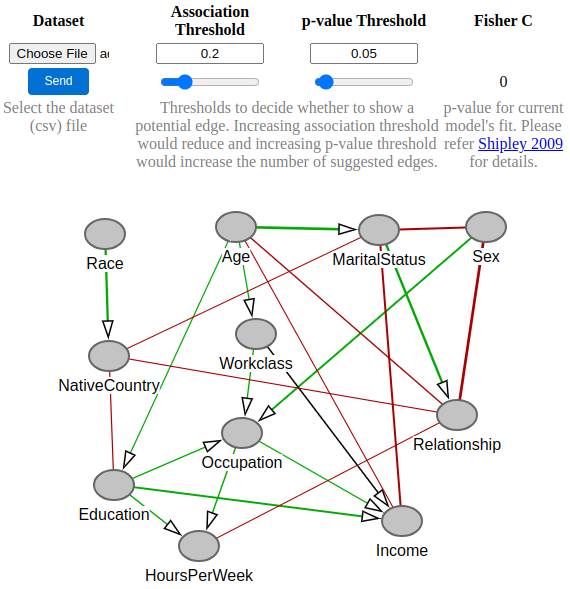
\includegraphics[scale=0.4]{../code/plots/web_tool_full.png}
	\caption{A screenshot of the web tool for constructing the model. Users
		can upload their dataset after which the tool creates an empty
		graph and shows all pair of variables which are associated in
		the model using undirected red edges with the strength of
		association represented using edge width. Users can then add
		edges to the model (shown in green). Unnecessary edges are shown in 
		black.}
	\label{fig:web}
\end{figure}

% \begin{figure}
% 	\centering
% 	\begin{subfigure}{0.5\textwidth}
% 		\includegraphics[scale=0.25]{../../presentations/2024_05_das/2.png}
% 	\end{subfigure}%
% 	\begin{subfigure}{0.5\textwidth}
% 		\includegraphics[scale=0.25]{../../presentations/2024_05_das/5.png}
% 	\end{subfigure}
% 	\caption{Screenshots of the web-tool. \todo[inline]{Insert screenshots of the web-tool}}
% \end{figure}

\section{Empirical Analysis}
\label{sec:empirical}

\begin{figure}[t!]
	\centering
	\begin{subfigure}{0.5\textwidth}
		\centering
		\includegraphics{../code/fig3/shd_ribbon.pdf}
		\caption{}
	\end{subfigure}
	\begin{subfigure}{0.5\textwidth}
		\centering
		\includegraphics{../code/fig3/sid_ribbon.pdf}
		\caption{}
	\end{subfigure}
	\caption{Comparison of PC and Hill-Climb Search algorithms against
		manually drawn DAGs using the assistance method. As PC and
		Hill-Climb Search return the Markov Equivalence Class (MEC), we
		use the best and worst scoring orientation of the MEC to get
		the range of values. The human drawn values are done for
		multiple accuracy values of the oracle.}
\end{figure}

\begin{figure}[t!]
	\begin{subfigure}{0.25\textwidth}
		\centering
		\includegraphics{../code/fig4/unexplained_effect.pdf}
		\caption{}
	\end{subfigure}%
	\begin{subfigure}{0.25\textwidth}
		\centering
		\includegraphics{../code/fig4/ll.pdf}
		\caption{}
	\end{subfigure}
	\caption{Plots showing improvements in fit of the model over iterations
	on the Adult income dataset. For the expert simulation an LLM is used
	for the edge orientations. (a) Shows using total unexplained effect that is the
	sum of effect size between variables that don't have an edge between them. (b)
	Shows the log-likelihood of the overall model.
	}
\end{figure}

We analyzed the performance of this manual approach by comparing it with two
automated algorithms: PC and Greedy Equivalence Search (GES). For the
comparison we use simulated data from a known DAG and compare how well the
algorithm is able to recover the original model using two metrics: Structural
Hamming Distance (SHD) and Structural Intervention Distance (SID). To simulate
the data, we start with a randomly generated DAG on $ 10 $ nodes and use linear
models with random effects to generate the data. 

We vary the edge probability of the DAG to generate DAGs with varying density.
We repeat the data generation $ 30 $ times for each density value for the DAG.
As both PC and Hill-Climb Search can only give us a CPDAG, we compare the
orientation of these CPDAG which result in the best and worst case scores on
SHD and SID.

To use our proposed approach, we need an expert to tell us the direction of the
edges. We simulated an expert using this assisted model construction approach,
we start with an empty model and take a greedy approach to add edges to this
model. At any point, we select the pair of variables that has significant
correlation and the highest unexplained correlation, i.e., highest conditional
association. We then use an oracle to decide the direction of the edge between
the variables. Given an accuracy of the oracle, $ \alpha $, the oracle either
gives the correct direction, incorrect direction, or returns None representing
that it does not know the direction.

\begin{equation}
	\begin{split}
		x &= \textnormal{rand}([0, 1]) \\
		O(\alpha) &= \begin{cases} 
			M \rightarrow Y, & \textnormal{if  } x <= \alpha \\
			\textnormal{rand}(M \rightarrow Y, M \leftarrow Y, None) & \textnormal{otherwise} \\
				\end{cases} \\
	\end{split}
\end{equation}

If the oracle returns None for any pair of variables, an edge between this pair
is not suggested to the oracle in future iterations. We also make sure that
only edges which do not form a cyclic in the graph are used to select the next
potential edge. After adding each edge, we also check if the p-value of any
existing edge shows independence. If that happens we remove that edge and
blacklist that edge, i.e., that edge is not prompted again during the run of
the algorithm. We repeat this procedure till the model explains all
correlations between the variables. There is a possibility that this greedy
expert gets stuck at incorrect graph structures as it does not do any
backtracking to fix its earlier mistakes. This procedure is outlined in the
Algorithm 1.
\todo[inline]{Show an algorithm of how this expert method is working}

\begin{verbatim}
	Input: Dataset $ D $ on variables $ \bm{X} $
	Output: Learned DAG G.
	
	function compute_effects(G):
		pvalues <- dict()
		effects <- dict()
		for X_i, X_j in X:
			if edge between X_i, X_j:
				p_values[(X_i, X_j)] <- pvalue(X_i, X_j, pa_{\bar{G}}(X_i) \cup pa_{\bar{G}}(X_j))
				effects[(X_i, X_j)] <- \phi(X_i, X_j, pa_{\bar{G}}(X_i) \cup pa_{\bar{G}}(X_j))
			else:
				p_values[(X_i, X_j)] <- pvalue(X_i, X_j, pa_{\bar{G}}(X_i) \cup pa_{\bar{G}}(X_j))
				effects[(X_i, X_j)] <- \phi(X_i, X_j, pa_{\bar{G}}(X_i) \cup pa_{\bar{G}}(X_j))
		return p_values, effects
	
	$ G $ <- Empty Graph
	p_values, effects <- compute_effects(G)
	while (p_values > p_thres, 
\end{verbatim}

\begin{algorithm}
	\KwData{Data set $ D $ on variables $ \bm{X} $, pthres, effectthres}
	\KwResult{The learned DAG: $ G $}
	\BlankLine
	$ G \leftarrow $ Empty Graph
\end{algorithm}


\subsection{Using LLMs as Experts}
Recently, there has been a lot of work towards using LLMs for causal discovery,
with tasks ranging from determining pairwise edge orientation
\citep{Kiciman2023, Jin2024} to full causal structure learning \citep{Naik2023,
Vashishtha2023} and counterfactual reasoning tasks\citep{Kiciman2023} (see
\citet{Liu2024} for an overview).

Since our approach utilizes expert knowledge to determine edge orientations, we
investigated the potential of using an LLM for this task. We applied our causal
discovery procedure with using Gemini 1.5 flash model as the expert. Our method
uses a greedy approach where the pair of variables with the highest unexplained
correlation is oriented first. The prompt used to determine the orientation is
provided in Appendix~\ref{section:llms}. Our LLM prompt utilizes variable
description to determine the edge orientation. We applied this approach to the
adult income dataset and the output is shown in Fig.~\ref{fig:adult_llm}. 

Unlike the other approaches to utilize LLM for doing full causal discovery, we 
used a combination of statistical tests and LLMs. This greatly reduces the
amount of information that we need from the LLM. Our approach is also able to 
ask exact questions about the variables unlike some of the other approaches.

\begin{figure}[t!]
	\centering
	\includegraphics[page=1]{fig5.pdf}
	\caption{DAG learned using the adult income dataset using an LLM (GEMINI-1.5-flash) as the expert.}
	\label{fig:adult_llm}
\end{figure}

\section{Conclusions}
Points:
\begin{itemize}
	\item As researchers prefer to anyways build models by hand, this is like a companion tool to help them in deciding the method.
	\item Solves all the $ 3 $ issues outlined in the introduction.
	\item Compared to other expert knowledge specification methods, users don't need to guess what information then need to provide as exact questions are asked. Also enables us to ask an LLM for it.
\end{itemize}

Future work:
\begin{itemize}
	\item Add latent variables; extend to ADMGs.
	\item Can potentially be combined with pairwise orientation methods.
	\item Improvements in the web-interface.
\end{itemize}

\bibliography{references}

\newpage

\onecolumn
\title{Expert-In-The-Loop Causal Discovery: Iterative Model Refinement Using Expert Knowledge \\ (Supplementary Material)}
\maketitle
\appendix

\section{Prompts Used for LLM}
\label{section:llms}

\begin{figure}[ht!]
	\centering
	\begin{verbatim}
You are an expert in Social Science. Following are the descriptions of two variables:

<A>: {description of variable A}
<B>: {description of variable B}

Which of the following two options is the most likely causal direction between these 
variables:

1. <A> causes <B>
2. <B> causes <A>

Return a single letter answer between the choices above; Do not provide any reasoning 
in the answer; Do not add any text formatting to the answer.
	\end{verbatim}
	\caption{Prompt used for the LLM. Here the variable descriptions are replaced with description provided in Fig.~\ref{fig:var_description}}
	\label{fig:prompt}
\end{figure}

\begin{figure}[ht!]
	\begin{verbatim}
          Age: The age of a person
    Workclass: The workplace where the person is employed such as Private industry, 
     	       or self employed
    Education: The highest level of education the person has finished.
MaritalStatus: The marital status of the person
   Occupation: The kind of job the person does. For example, sales, craft repair, 
   		clerical.
 Relationship: The relationship status of the person.
         Race: The ethnicity of the person.
          Sex: The sex or gender of the person.
 HoursPerWeek: The number of hours per week the person works.
NativeCountry: The native country of the person.
       Income: The income i.e. amount of money the person makes.
	\end{verbatim}
	\caption{Variable descriptions used for prompting the LLM}
	\label{fig:var_description}
\end{figure}

\section{A Generalized Measure of Conditional Association}
\label{sec:mixed_association}

In the previous section, we discussed how different types of variables require
different measures of conditional association. However, there is no unified
measure that handles mixed data. In this section, we introduce a measure of conditional
association for mixed data by extending the concept of partial correlation
coefficient (commonly used for continuous variables) to mixed data. Similar to
partial correlation coefficient, our method integrates a mixed data
residualization method \citep{Ankan2023} with Pillai's Trace
\citep{Pillai1955}, a multivariate measure of association based on canonical
correlations.
 
Given a dataset $ D = (x, y, \bm{z}) $ on variables $ X $, $ Y $, and $ \bm{Z}
$, our goal is to estimate the conditional association $ \phi_{X, Y; \bm{Z}} $. 
In the first step, we compute the residuals $ R_X $ and $ R_Y $ for variables
$ X $ and $ Y $ respectively. Depending on the type of variable the residual
is computed as follows:

\begin{enumerate}
	\item \textbf{Continuous:} We train a model, $ E_X: x \sim
		\bm{z} $. The residuals are then computed by taking the difference
		between the true and the predicted values using $ E_X $. 
		$$ R_{x_i} = x_i - E_X(\bm{z}_i) $$
	\item \textbf{Ordinal:} We start by training a probability estimator, $
		p_X: x \sim \bm{z} $, and then use the estimated probabilities, 
		$ \hat{p}_X(x) $ to compute the residuals:
		$$ R_{x_i} = \hat{p}_X(X < x_i) - \hat{p}_X(X > x_i) $$
	\item \textbf{Categorical:} We again start by training a probability
		estimator $ p_X: x \sim \bm{z} $, and obtain probability
		estimates $ \hat{p}_X: p_X(\bm{z}) $. Next, we dummy encode the
		categorical variable, resulting in a binary vector and then
		compute the residuals as follows: 
		$$ R_{x_i} = x_i - \hat{p}_X(\bm{z}_i) $$
\end{enumerate}

We have the option here to choose the estimators based on the characteristics
such as distribution, type of relationship, and so on of our dataset.
Non-parametric ensemble estimators such as Random Forest and XGBoost are robust 
for diverse data types and complex relationships. For linear relationships,
simpler models such as linear regression and its variants may suffice.

We repeat the above residualization step for both the variables $ X $ and $ Y $
obtaining residual matrices $ R_x $ and $ R_y $. The type of variable determines
the shape of these matrices. If the variable is continuous or ordinal, the 
residual matrix is of shape $ (n \times 1 ) $ and if the variable is categorical,
we get a residual matrix of shape $ (x \times (k - 1)) $, where $ k $ is the number
of categories of the variable.

The second step is to quantify the association between these residual matrices.
For this purpose we use canonical correlations \citep{Hotelling1936} that have been widely used to
measure the association between sets of random variables.

\begin{definition}
	Given two sets of random variables $ \bm{U} = (U_1, U_2, \cdots, U_p) $
	and $ \bm{V} = (V_1, V_2, \cdots, V_q) $, canonical correlation between
	them, $\rho_{\bm{U}, \bm{V}} $ is defined as:
		
	\begin{equation}
		% \nu_{\bm{U}, \bm{V}}= \max_{a, b} \mathrm{corr}(a^T \bm{U}, b^T \bm{V})
		\rho_{\bm{U}, \bm{V}} = \max_{a, b} \frac{a^T \Sigma_{\bm{UV}} b}{\sqrt{a^T \Sigma_{\bm{UU}} a \cdot b^T \Sigma_{\bm{VV}} b}}
	\end{equation}

	where $ a $ and $ b $ are vectors of coefficients that maximize the correlations
	between the linear combinations of $ a^T \bm{U} $ and $ b^T \bm{V} $.
\end{definition}

Canonical correlations generalize the concept of correlation coefficients to
multi-dimensional variables. It finds orthogonal linear transformations $ a $
and $ b $ that maximized the correlation between the transformed variables $
a^T \bm{U} $ and $ b^T \bm{V} $. This yields a vector of correlation
coefficient values of size $ \min(p, q) $, representing the correlation
coefficient of each pair of transformed variables. Notably, Pearson's
correlation coefficient is a special case of canonical correlations when $ p =
q = 1 $.

Several measures of association have been derived from canonical correlations, such as:
\begin{itemize}
	\item Wilks' Lambda: $\Lambda = \prod_{i}^{\min(p, q)} (1 - \rho_i^2) $
	\item Roy's Largest Root: $ \theta = \max_i(\rho_i^2) $
	\item Pillai's Trace: $ \tau = \sum_{i=1}^{\min(p, q)} \rho_i^2 $
\end{itemize}

We use a normalized version of Pillai's Trace for our purpose, given as:

\begin{equation}
	\tau_{X, Y; \bm{Z}} = \frac{1}{\min(\rvert R_x \rvert, \rvert R_y \rvert)}
	\sum_{i=1}^{\min(\rvert R_x \rvert, \rvert R_y \rvert)} (\rho_{R_x, R_y})_i^2
\end{equation}


We use Pillai's Trace because: 1) It uses all the canonical correlation values,
capturing the full extent of association, 2) Its interpretation is similar to
Pearson's correlation coefficient, i.e., $ 0 $ signifies no association and $ 1
$ signifies perfect linear relationship. We use a normalized version because
when comparing between pair of variables with different number of categories.
Our proposed measure has several desirable properties that make it well-suited
for our application:

\begin{enumerate}
	\item \textbf{Bounded: } The measure is bounded between $ 0 $ (no
		association) to $ 1 $ (perfect linear association), simplifying
		interpretation.
	% \item \textbf{Independent of Sample Size: } 
	\item \textbf{Invariant to the Dummy Encoding: } For categorical
		variables, residuals are computed using dummy encoding. Since
		canonical correlations identifies linear combinations across
		columns, this measure is invariant to the specific dummy
		encoding scheme used.
	\item \textbf{Equivalent to Partial Correlation for Continuous Variables: }
		When both $ X $ and $ Y $ are continuous variables, our measure
		is equivalent to the absolute value of partial correlation coefficient.
	\item \textbf{Equivalent to polychoric and polyserial correlation for
			ordinal and continuous variables: }
		Under the assumption that the ordinal variable is generated by
		discretizing an underlying gaussian continuous variable, this
		effect size is equivalent to polychoric and polyserial
		correlation. As both of them recover the Pearson correlation
		coefficient.
		\todo[inline]{Verify if this is correct}
	\item \textbf{Related to Cram\'er's V: } 
\end{enumerate}

In essence, our measure of conditional association extends existing metrics to mixed data, providing 
a unified measure that is interpretable.

\end{document}
